\documentclass[12pt]{article}

\usepackage[margin=1in]{geometry}	% margin settings
\usepackage{amsfonts, amsmath, amssymb}	% symbols and environments for math
%\usepackage[none]{hyphenat}	% prevent hyphenation of text
\usepackage{graphicx}
\usepackage{import}
\usepackage{float}
\usepackage{hyperref}	% provide ability to have pdf links
\usepackage{xcolor}

\setlength{\parindent}{0em}	% indentation of new paragraph
\setlength{\parskip}{0.5em}	% spacing between paragraphs
\renewcommand{\baselinestretch}{1}	% line-spacing

%opening
\title{How To Write With Me}
\author{H.W. Jordaan and H. Kamper}

\begin{document}

\maketitle

\section*{What does this guide contain?}
This document aims to transfer the picture of the perfect academic research report and how to construct that with a supervisor.
Of course each supervisor is different and might have his/her own pet peeves.
You need to adjust to your specific boss.

The majority of this document should not be read from the start to the end, but should rather serve be referred to while writing and want advice in how to do a certain thing.
Each section of this guide will try and cover a single question or component.

\section*{What is a good report for you?}
This guide will never be able to absorb all the questions you will have during writing.
It is important to note that you are not the first person who is trying to write a report or article.
There are many reports/articles you can use as examples of what to do or even what you did not like.
It means that while you are reading an article or resource in preparation for your work that you make notes on the side just highlighting the style and language aspects of the paper.
You do not even have to read through an entire paper to be able to make at least one comment.

I would define a good report as:
\begin{itemize}
	\item To the point and theme; do not put stuff in just for the sake of content; remember what is the main them of your writing.
	\item Something that reads easily; you do have to reread a certain paragraph or section two or three times.
	\item The report is neat;  tables and figures are good and legible.
	\item Accurate;  stuff are done consistently (headings, capitalisation, size of figures ect.) and with very few errors such as typos or spelling mistakes.
\end{itemize}

\section*{Where should I start?}
The report should be easy to read for the examiner and other readers.
One way to do it is to ensure that your report has some kind of \textit{story}.
Basically you should be able to describe the flow of your report in a few sentences without any large jumps.
The reader needs to be able to easily follow your thought and your process from start to end.

Here is a suggested workflow to get you started with your report/article:
\begin{itemize}
	\item Write down the main theme of your report/article.  This should not be more than two sentences.
	\item Start a \textit{Table of Contents} and identify first the major chapters and try and go down to at least a section level.
	\item Start creating content and start with a technical chapter or section, not the introduction or literature study.
	\item Keep going!
\end{itemize}

\section*{We do not clap hands for basics}
We all make mistakes and try to learn from them.
There are some mistakes that does make your supervisor very sad.
Here are some basics that is expected when a student gives any draft or piece of writing:
\begin{itemize}
	\item Spelling mistakes.  With word processors, editors and tools (Grammarly) of today, there is no excuse for spelling mistakes.
	\item If you receive feedback on a previous draft, it expected that you worked the recommendations into the entire manuscript.  Often the mistake is only fix the first time it occurs.  It is assumed that you will fix all occurrences of this mistake throughout the entire document.
	\item If you have a figure or table, you need to refer to it and describe it in the text.
	\item Please learn the difference between \textit{its} and \textit{it's}.
	This is probably the most common error that is encountered in all forms of writing.
	Yes, even in journal papers.
\end{itemize}

\section*{What is a literature study?}
A literature study aims to define and show what other people have done to try and solve the main problem which you introduced in your introduction.
Many students get the function of this chapter correct and quickly become simply either a dump of a lot of references or worse just any content is used somewhere to the document that is not even related to the main problem.

If your main theme to control a pendulum, your literature study should be focused on how other people tackle the control of a pendulum.
The literature on bearings should not be present in the main literature study even if you might need it later in your report.

At the end of the literature study, you should be able to analyse or comment on what and how other people are solving a similar problem.  You will be using these observations and conclusions to base your design choices for the rest of your report.

Be wary of writing the literature study in a boring tone such as Guy A did this and this.  This remains a study and should be a refinement and a worked version of the content of the source.

This chapter is normally difficult to write well, i.e. not boring and to the point.  It is suggested to start early in the writing process with the chapter but to always keep in on the side while writing other chapters.


\section*{How to handle mathematics}
There are two way in handling mathematical equations in your text.
Either you can handle it as a figure and see it separate of the text and refer to it in the text, or the other option is to see it part of the sentence.
Your choice is a function of the amount of mathematics to foresee you would have in your text.
If you expect a lot of mathematical derivation it will become a hindrance if the reader have to follow a referral to a specific equation in the text.

If mathematics becomes part of your sentences it should have all the required punctuation.
Here is an example:

The area of a circle can be calculated by:
\begin{equation}
A = \pi r^{2},
\end{equation}
where $r$ is the radius of the circle.

Other important thing to note:
\begin{itemize}
	\item Always introduce your variables the first time you use them in your text.
	Do not be only dependent on your nomenclature to define the meaning of the variables to your reader.
	
	\item Consistent mathematical symbols. If $x$ is used to represent something in Section 1, then $x$ should not be used for something else in Section 3.
	Sometimes it is difficult to be entirely consistent (this is often the case in bigger documents like a thesis).
	But then you need to tell the reader clearly that you are being somewhat loose with your notation.
	
	\item We sometimes use ``proper'' words or abbreviations to denote an operation within a mathematical expression.
	For instance, we use ``max'' to denote maximisation or ``log'' to indicate that we are taking the logarithm. In these cases, the operation should be denoted with an upright font, e.g. $\max(x)$, not $max(x)$.
	The latter implies a multiplication of variables, i.e. $m\cdot a\cdot x$. You should also use an upright font if you use a word as a sub- or superscript to denote some properties of a variable, e.g. you should write $y_{\text{pair}}$, not $y_{pair}$.
\end{itemize}

\section*{What makes a good picture?}
A picture says a thousand words, and it easy to describe and write with you have a picture that you can refer.
The opposite is also true, which is that if the picture is bad the reader will not enjoy the report.

Pictures are a great way to break a page and prevent it in becoming a sea of text.
A reader will be more likely to read the page if there is a picture somewhere on the page.
Use this to bring important concepts to the reader, such as conceptual design, architectures.
An example of a good picture is shown in Figure \ref{fig:cameraslam2comp}.

\begin{figure}
	\centering
	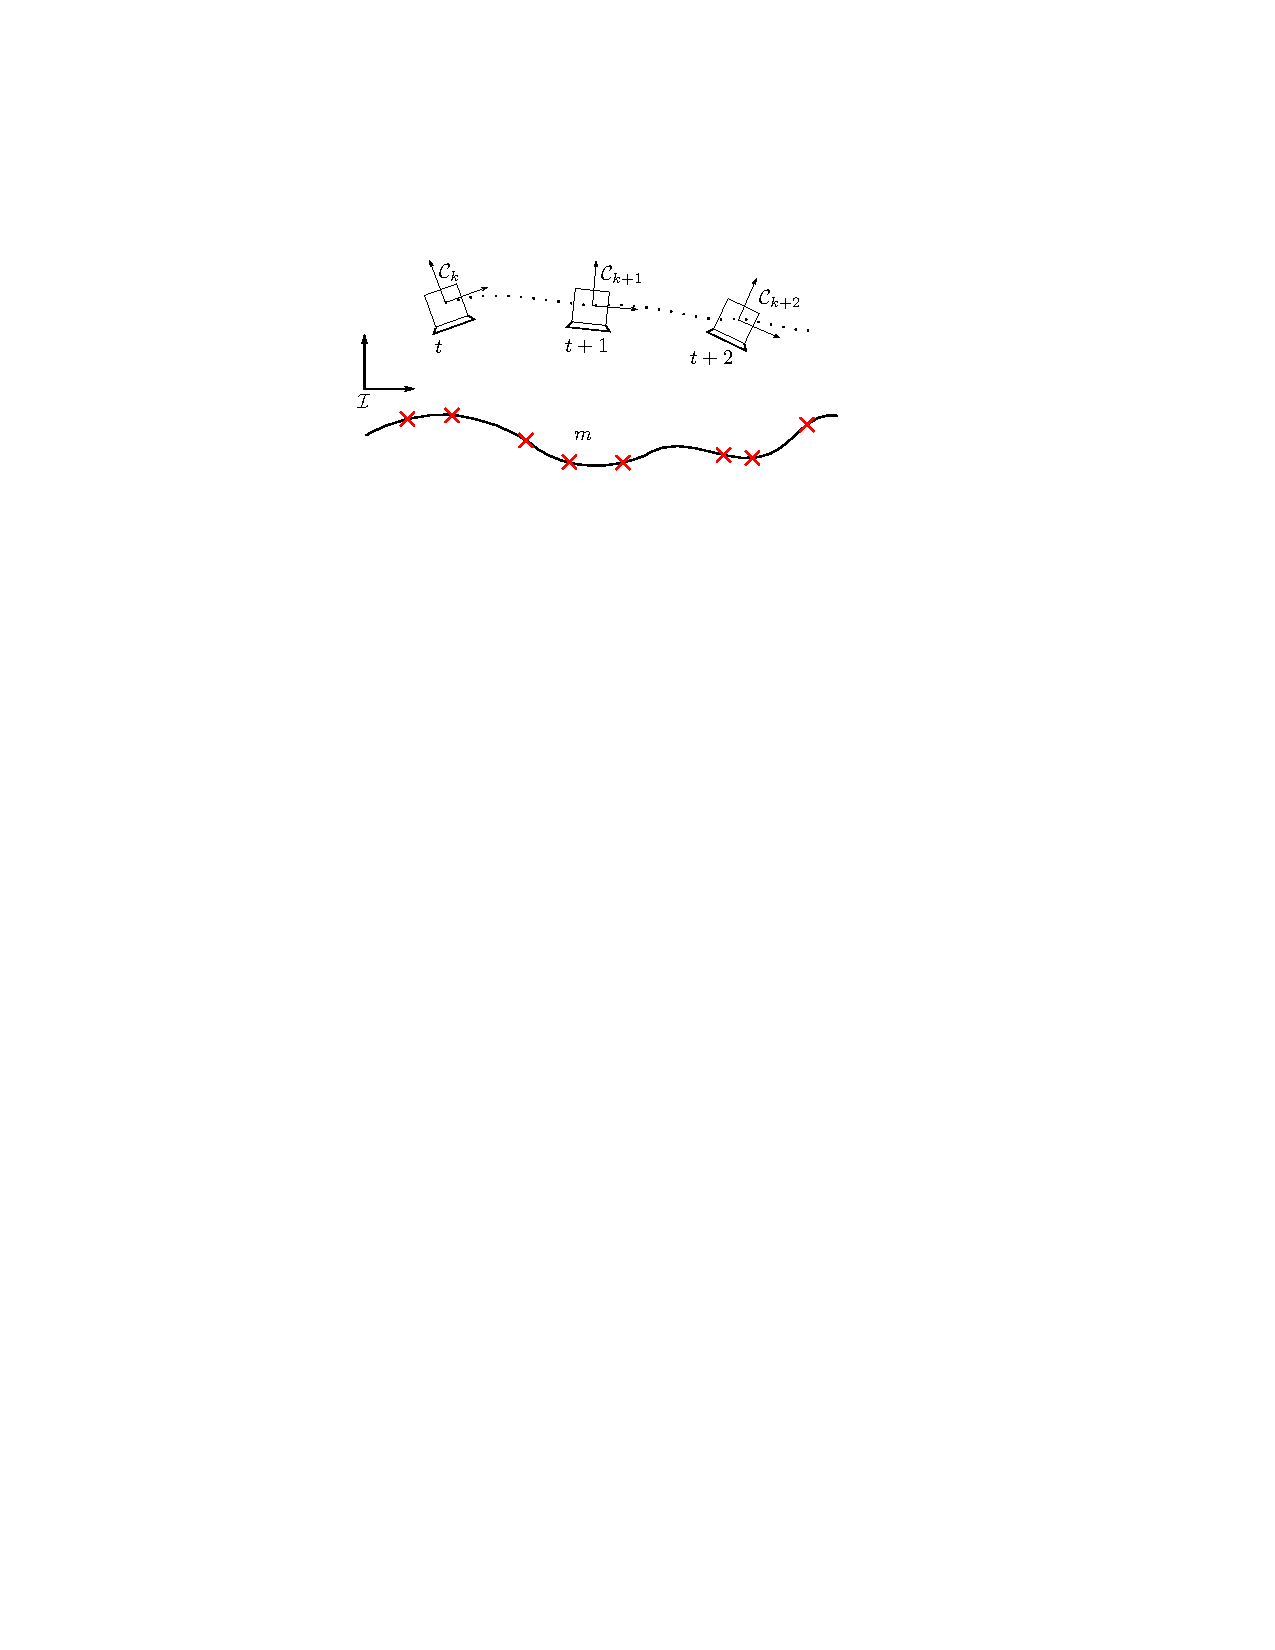
\includegraphics[width=0.7\linewidth]{figures/CameraSLAM2_comp}
	\caption{Illustration of the classic SLAM problem, where a robot moves through an initially unknown environment. Landmarks, indicated by the red crosses, are observed and used to build a map, m, of the environment. This map is used by the robot to localise itself in the map. The sensor reference frame (CRF) is denoted by $\mathcal{C}$.}
	\label{fig:cameraslam2comp}
\end{figure}

A few other things to note:
\begin{itemize}
	\item Quality of image; ensure that the quality of the rendered image is good, vector based graphics are ideal.
	\item Try and keep the pictures simple; do not go over the board with textures and colours if it is not really required.
	\item If there are text and labels, try and make them a similar size which are found in the rest of the text.
	\item Try to place figures close to where they are first mentioned.
	\item Try and prevent a picture to encompass the entire page.
	\item If you do not refer to the picture then it should not be there.
	\item You can not assume that the reader understands the picture.
	There should always be text describing the image.
	\item Ensure that the caption of the image is complete and that the reader can understand what is in the picture from the caption.
\end{itemize}

\section*{What makes a good graph?}
Graphs are extremely important and in many cases are the main form in which results are delivered.


There are a number of common errors that are made in graphs:
\begin{itemize}
	\item Label text is too small and not legible.
	\item Graph lines are too thin.
	\item The graph window is too long.
	Sometimes better to break the time window/scenario up into smaller graphs so that transients are more visible.
\end{itemize}

An example of a good graph is shown in Figure \ref{fig:good_graphs}.

\begin{figure}
	\centering
	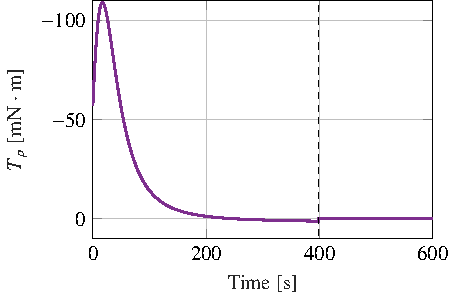
\includegraphics[width=0.5\linewidth]{figures/LdCont_T_p}
	\caption{The pulley deployment actuator torque for the active deployment rate controller.}
	\label{fig:good_graphs}
\end{figure}

\section*{What makes a good table?}

\section*{What is expected from references?}

\section*{Questions still to be covered}
\begin{itemize}
	\item 
\end{itemize}



\end{document}